\documentclass[12pt,aspectratio=169]{beamer}

\mode<presentation>
{
  \usetheme{Singapore}
  \setbeamersize{text margin left=.5cm,text margin right=.5cm}
%  \setbeamertemplate{navigation symbols}{} % suppress nav bar
%  \setbeamercovered{transparent}
}
\usefonttheme{professionalfonts}
\usepackage{graphicx}
\usepackage{tikz}
\usepackage{mathpazo}
\usepackage[scaled]{helvet}
\usepackage{xcolor,colortbl}
\usepackage{hyperref}
\usepackage{siunitx}


\sisetup{
  number-math-rm=\mathnormal
}
%\sisetup{detect-all}


\title[Waves]{Topic 17: Mechanical Waves}
\subtitle{Advanced Placement Physics}
\author[TML]{Dr.\ Timothy Leung}
\institute{Olympiads School}
\date{Spring 2019}
%\date{Summer 2018}

\newcommand{\pic}[2]{\includegraphics[width=#1\textwidth]{#2}}
\newcommand{\eq}[2]{\vspace{#1}{\Large\begin{displaymath}#2\end{displaymath}}}


\begin{document}


\begin{frame}
  \titlepage
\end{frame}



\section{Mechanical Waves}
\begin{frame}
  \frametitle{What is a wave?}
  \begin{itemize}
  \item When a disturbance (vibration) causes vibrations in its vicinity, a
    wave is created
  \item A wave transfers energy through a medium
    \begin{itemize}
    \item The medium vibrates and have a net displacement of zero.
    \item Each particle vibrates instead of moving horizontally, and the
      vibration get transferred to the next particle.
    \item Electromagnetic (''EM'') waves are the only kind that does not
      require a medium
    \end{itemize}
  \end{itemize}
\end{frame}



\begin{frame}{Features of a Wave}
  \begin{itemize}
  \item The \emph{highest} point of the wave is called a \textbf{crest} or
    \textbf{peak}, while
  \item The \emph{lowest} point in the wave is called a \textbf{trough}.
  \item The \textbf{wavelength} $\lambda$ is the shortest distance between two
    points in the medium that are in phase. The easiest way to measure
    wavelength is from crest to crest, or from trough to trough.
  \end{itemize}
  \begin{center}
    \vspace{-.4in}\pic{.8}{sine-wave1.png}
  \end{center}
\end{frame}


\begin{frame}{The Wave Equation}
  The mechanical wave as we know it is the solution to a second-order partial
  differential equation\footnote{The equation is \emph{second order} because
    it contains second derivatives, and \emph{partial} because it involves
    partial derivatives with respect to both space $x$ and time $t$.}:
  
  \eq{-.2in}{
    \frac{\partial^2 u}{\partial t^2}=c^2\frac{\partial^2 u}{\partial x^2}
  }

  subject to initial condition.
\end{frame}


\begin{frame}{Equation of a Traveling Wave}
  The solution to the wave equation is a \textbf{harmonic wave} that can be
  described as a sinusoidal function that oscillates in both space $x$ and time
  $t$:
  
  \eq{-.2in}{
    \boxed{u(x,t)=A\sin(kx-\omega t)}
  }
  \begin{center}
    \begin{tabular}{l|c|l}
      \rowcolor{pink}
      \textbf{Quantity} & \textbf{Symbol} & \textbf{SI Unit} \\ \hline
      Displacement of the medium  & $u$ & \si{\metre} (meters)\\
      Amplitude of the wave       & $A$ & \si{\metre} (meters)\\
      Wave number                 & $k$ & \si{\per\metre} (per meter)\\
      Distance from the source    & $x$ & \si{\metre} (meters)\\
      Time                        & $t$ & \si{\second} (seconds)\\
      Angular frequency           & $\omega$ & \si{\per\second} (per second)
    \end{tabular}
  \end{center}
\end{frame}


\begin{frame}{Equation of the Wave}
  \eq{-.1in}{
    \boxed{y(x,t)=A\sin(kx-\omega t)}
  }

  If the wave is generated by a mass on a spring, then $k$ is the spring
  constant of the spring. It is related to the wavelength $\lambda$ by:
  
  \eq{-.2in}{
    k=\frac{2\pi}{\lambda}
  }

  \vspace{-.1in}The angular frequency (angular velocity) is related to the
  frequency $f$ and period $T$ of the wave by:

  \eq{-.35in}{
    \omega=\frac{2\pi}{T}=2\pi f
  }
\end{frame}



\begin{frame}{Universal Wave Equation}
  When combining the wave number and angular frequency, we can find that
  the speed of a wave is the product of the wavelength and the frequency:

  \eq{-.2in}{
    \boxed{v = f\lambda}
  }
  \begin{center}
    \begin{tabular}{l|c|l}
      \rowcolor{pink}
      \textbf{Quantity} & \textbf{Symbol} & \textbf{SI Unit} \\ \hline
      Speed         & $v$       & \si{m/s} (meters per second) \\
      Frequency     & $f$       & \si{\hertz} (hertz)\\
      Wavelength    & $\lambda$ & \si{\metre} (meters)
    \end{tabular}
  \end{center}
  The universal wave equation applies to \emph{all} waves. For sound waves,
  $v=v_\mathrm{sound}$; for electromagnetic waves $v=c$.
\end{frame}


\begin{frame}{Why Sine and Cosines}
  French mathematician Joseph Fourier showed that \emph{all} periodic functions
  can be represented as an infinite series of $\sin$ and/or $\cos$ functions:

  \vspace{-.35in}{\Large
    \begin{align*}
      f(x)=&a_1\sin(x)+a_2\sin(2x)+a_3\sin(3x)+\ldots+\\
      &b_1\cos(x)+b_2\cos(2x)+b_3\cos(3x)+\ldots\\
      =&\sum_{n=1}^{\infty}a_n\sin(nx)+\sum_{n=1}^{\infty}b_n\cos(nx)
    \end{align*}
  }

  The sum is called the \textbf{Fourier series}. Depending on the shape of the
  wave, some coefficients $a_n$ and $b_n$ are zeros. This part is particularly
  important to sound waves.
\end{frame}


\begin{frame}{Frequency and Speed of A Wave}

  Frequency of A Wave ($f$)
  \begin{itemize}
  \item The number of complete wavelengths that pass a point in a given amount
    of time
  \item Unit: hertz (\si{\hertz})
  \item Same as the frequency of the disturbance that generated the wave
  \item\textbf{Does not depend on the medium}, only the source that produced
    the wave
  \end{itemize}

  \vspace{.2in}Speed of A Wave ($v$)
  \begin{itemize}
  \item The speed at which the wave fronts are moving
  \item\textbf{Depends only on the medium}, not the source that produced the
    wave
  \end{itemize}
\end{frame}



\begin{frame}{Making a Square Wave with Sine Waves}
  \begin{columns}
    
    \column{.6\textwidth}
    \centering
    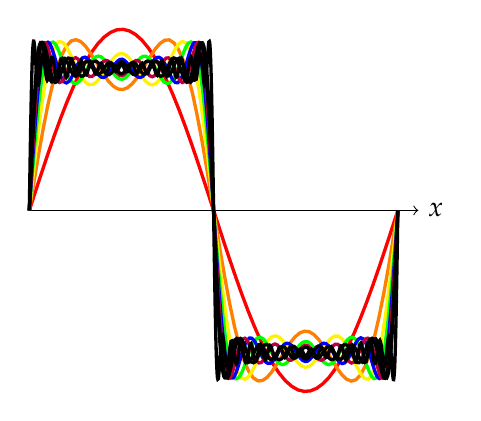
\begin{tikzpicture}[xscale=.013,yscale=2.3]
      \draw[->](0,0)--(380,0) node[pos=1,right]{$x$};
      \uncover<1>{
        \draw[samples=60,domain=0:360,red,very thick]plot({\x},{sin(\x)});
      }
      \uncover<2>{
        \draw[samples=80,domain=0:360,orange,very thick]
        plot({\x},{sin(\x)+1/3*sin(3*\x)});
      }
      \uncover<3>{
        \draw[samples=100,domain=0:360,yellow,very thick]
        plot({\x},{sin(\x)+1/3*sin(3*\x)+1/5*sin(5*\x)});
      }
      \uncover<4>{
        \draw[smooth,samples=140,domain=0:360,green,very thick]
        plot({\x},{sin(\x)+1/3*sin(3*\x)+1/5*sin(5*\x)+1/7*sin(7*\x)});
      }
      \uncover<5>{
        \draw[smooth,samples=160,domain=0:360,blue,very thick]
        plot({\x},
        {sin(\x)+1/3*sin(3*\x)+1/5*sin(5*\x)+1/7*sin(7*\x)+1/9*sin(9*\x)});
      }
      \uncover<6>{
        \draw[smooth,samples=160,domain=0:360,purple,very thick]
        plot({\x},
        {sin(\x)+1/3*sin(3*\x)+1/5*sin(5*\x)+1/7*sin(7*\x)+1/9*sin(9*\x)+
          1/11*sin(11*\x)});
      }
      \uncover<7>{
        \draw[smooth,samples=200,domain=0:360,very thick]
        plot({\x},
        {sin(\x)+1/3*sin(3*\x)+1/5*sin(5*\x)+1/7*sin(7*\x)+1/9*sin(9*\x)+
          1/11*sin(11*\x)+
          1/13*sin(13*\x)});
      }
      \uncover<8>{
        \draw[smooth,samples=200,domain=0:360,very thick]
        plot({\x},
        {sin(\x)+1/3*sin(3*\x)+1/5*sin(5*\x)+1/7*sin(7*\x)+1/9*sin(9*\x)+
          1/11*sin(11*\x)+
          1/13*sin(13*\x)+
          1/15*sin(15*\x)});
      }
      \uncover<9>{
        \draw[smooth,samples=350,domain=0:360,very thick]
        plot({\x},
        {sin(\x)+1/3*sin(3*\x)+1/5*sin(5*\x)+1/7*sin(7*\x)+1/9*sin(9*\x)+
          1/11*sin(11*\x)+ 1/13*sin(13*\x)+ 1/15*sin(15*\x)+ 1/17*sin(17*\x)+
          1/19*sin(19*\x)+
          1/21*sin(21*\x)+ 1/23*sin(23*\x)+ 1/25*sin(25*\x)+ 1/27*sin(27*\x)+
          1/29*sin(29*\x)+
          1/31*sin(31*\x)+ 1/33*sin(33*\x)+ 1/35*sin(35*\x)+ 1/17*sin(37*\x)+
          1/39*sin(39*\x)});
      }
    \end{tikzpicture}

    \column{.35\textwidth}
    \uncover<1->{
      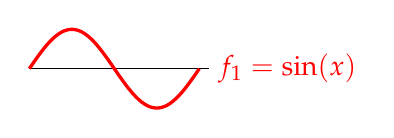
\begin{tikzpicture}[xscale=.006,yscale=.5]
        \draw(0,0)--(380,0) node[pos=1,right]{\color{red}$f_1=\sin(x)$};
        \draw[samples=60,domain=0:360,red,very thick] plot({\x},{sin(\x)});
      \end{tikzpicture}
    }
    \uncover<2->{
      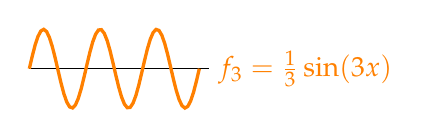
\begin{tikzpicture}[xscale=.006,yscale=.5]
        \draw(0,0)--(380,0) node[pos=1,right]
             {\color{orange}$f_3=\frac{1}{3}\sin(3x)$};
        \draw[samples=60,domain=0:360,orange,very thick] plot({\x},{sin(3*\x)});
      \end{tikzpicture}
    }
    \uncover<3->{
      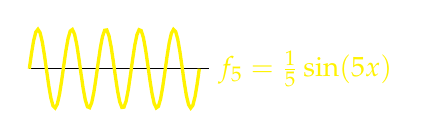
\begin{tikzpicture}[xscale=.006,yscale=.5]
        \draw(0,0)--(380,0) node[pos=1,right]
             {\color{yellow}$f_5=\frac{1}{5}\sin(5x)$};
        \draw[samples=80,domain=0:360,yellow,very thick] plot({\x},{sin(5*\x)});
      \end{tikzpicture}
    }
    \uncover<4->{
      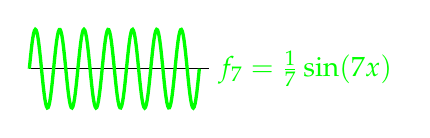
\begin{tikzpicture}[xscale=.006,yscale=.5]
        \draw(0,0)--(380,0) node[pos=1,right]
             {\color{green}$f_7=\frac{1}{7}\sin(7x)$};
        \draw[samples=200,domain=0:360,green,very thick] plot({\x},{sin(7*\x)});
      \end{tikzpicture}
    }
    \uncover<5->{
      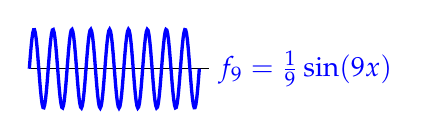
\begin{tikzpicture}[xscale=.006,yscale=.5]
        \draw(0,0)--(380,0) node[pos=1,right]
             {\color{blue}$f_9=\frac{1}{9}\sin(9x)$};
        \draw[samples=200,domain=0:360,blue,very thick] plot({\x},{sin(9*\x)});
      \end{tikzpicture}
    }
  \end{columns}
\end{frame}

\begin{frame}{Fourier Series and Harmonic Frequencies}
  \begin{center}
    \vspace{-.3in}
    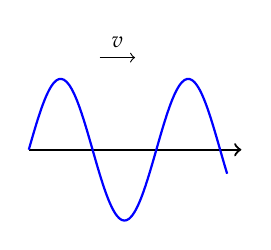
\begin{tikzpicture}[scale=.9]
      \draw[->,thick](0,0) --(3,0);
      \draw[->](1,1.3)--(1.5,1.3) node[midway,above]{\footnotesize $v$};
      \draw[thick,blue,smooth,samples=80,domain=0:2.8] plot({\x},{sin(200*\x)});
    \end{tikzpicture}
    \hspace{.15in}
    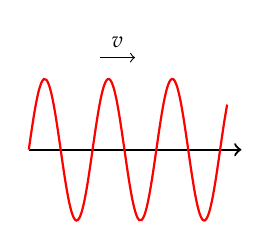
\begin{tikzpicture}[scale=.9]
      \draw[->,thick](0,0) --(3,0);
      \draw[->](1,1.3)--(1.5,1.3) node[midway,above]{\footnotesize $v$};
      \draw[thick,red,smooth,samples=80,domain=0:2.8] plot({\x},{sin(400*\x)});
    \end{tikzpicture}
    \hspace{.15in}
    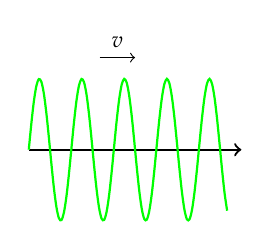
\begin{tikzpicture}[scale=.9]
      \draw[->,thick](0,0) --(3,0);
      \draw[->](1,1.3)--(1.5,1.3) node[midway,above]{\footnotesize $v$};
      \draw[thick,green,smooth,samples=80,domain=0:2.8]
      plot({\x},{sin(600*\x)});
    \end{tikzpicture}
  \end{center}

  \vspace{-.2in}
  \begin{itemize}
  \item The first wave---with the longest wavelength and lowest
    frequency---is called the \textbf{fundamental frequency}, or
    \textbf{first harmonic}
  \item The second term has half the wavelength and twice the frequency. It's
    called the \textbf{second harmonic}, the \textbf{first overtone}
  \item Also, third, fourth, fifth\ldots harmonics
  \end{itemize}
\end{frame}



\begin{frame}{Harmonic Frequencies}
    Every whole-number multiples of the fundamental frequency $f_1$ is its
    harmonic frequency, i.e.\ the $n$-th harmonic is:

    \eq{-.25in}{
      \boxed{f_n=nf_1}\quad n=1,2,3,\ldots
    }
    For sound waves, when a musical instrument produces a sound that has, the
    frequency that is ``heard'' is the fundamental frequency
\end{frame}



\begin{frame}{Two Kinds of Waves}
  \begin{center}
    \pic{.6}{main-qimg.png}
  \end{center}
  \begin{enumerate}[a.]
  \item\vspace{-.2in}\textbf{Longitudinal wave}
    \begin{itemize}
    \item Vibration is parallel to the direction of the motion of the wave
    \item Example: sound waves
    \end{itemize}
  \item\textbf{Transverse wave}
    \begin{itemize}
    \item Vibrations occur right angles to the direction of the wave
    \item Example: electromagnetic waves
    \end{itemize}
  \end{enumerate}
\end{frame}

\begin{frame}{Wave Simulation}
  A helpful simulation can be found on the PhET website at University of
  Colorado.
  \begin{center}
    \textbf{Click for external link:}\\
    \href{https://phet.colorado.edu/sims/html/wave-on-a-string/latest/wave-on-a-string_en.html}
         {wave on a string simulation}
  \end{center}
\end{frame}



\begin{frame}{Wave on a String}
  The speed of a traveling wave on a stretched string is determined by:

  \eq{-.2in}{
    \boxed{v=\sqrt{\frac{F_T}{\mu}}}
    \quad\text{\normalsize where}\quad
    \boxed{\mu=\frac{m}{L}}
  }
  \begin{center}
    \begin{tabular}{l|c|l}
      \rowcolor{pink}
      \textbf{Quantity} & \textbf{Symbol} & \textbf{SI Unit} \\ \hline
      Wave speed    & $v$    & \si{m/s} (meters per second) \\
      Tension       & $F_T$  & \si{\newton} (newtons)\\
      Linear mass density & $\mu$ & \si{\kilo\gram/\metre} (kilograms per meter)
      \\
      Mass of the string & $m$    & \si{\kilo\gram} (kilograms)\\
      Length of the string & $L$ & \si{\metre} (meters)
    \end{tabular}
  \end{center}
\end{frame}


\begin{frame}{Power Transmitted by a Harmonic Wave}
  Then the power transmitted by a harmonic wave is through a traveling wave on
  a string is determined by the linear mass density $\mu$, the angular frequency
  $\omega$, amplitude $A$ and wave speed $v$:

  \eq{-.2in}{
    \boxed{P=\frac{1}{2}\mu\omega^2A^2v}
  }
\end{frame}
%
%
%\begin{frame}
%  \frametitle{The Decibel}
%  The decibel is defined as by the intensity of sound $I$ compared to the
%  \emph{threshold of hearing} intensity $I_0$:
%  
%  \eq{-.3in}{
%    \boxed{\beta=10\log_{10}\left[\frac{I}{I_0}\right]}
%    \;\;\text{\normalsize where}\;\; I_0=\SI{e-12}{\watt/\metre^2}
%    \;\;\text{\normalsize and}\;\;
%    \boxed{I=\frac{P_\mathrm{ave}}{4\pi r^2}}
%  }
%  \begin{center}
%    \begin{tabular}{l|c|l}
%      \rowcolor{pink}
%      \textbf{Quantity} & \textbf{Symbol} & \textbf{SI Unit} \\ \hline
%      Intensity of sound  & $\beta$ & \si{\decibel} (decibels)\\
%      Intensity of sound  & $I$ & \si{W/m^2} (watts per square meters)\\
%      Threshold intensity & $I_0$ & \si{W/m^2} (Watts per square meters)\\
%      Average power of the source & $P_\mathrm{ave}$  & \si{\watt} (watts)\\
%      Distance from the source & $r$  & \si{\metre} (meters)
%    \end{tabular}
%  \end{center}
%  The \emph{threshold of pain} for human ears is defined at \SI{120}{\decibel}.
%\end{frame}


\begin{frame}{Reflection of a Wave at a Boundary}
  \begin{columns}
    \column{.5\textwidth}
    When a wave on a string reflects at a boundary, how the reflected wave looks
    depends on the type of boundary
    \begin{itemize}
    \item At a \emph{fixed end} (left), the reflected wave is \emph{inverted},
      i.e.\ a crest becomes a trough
    \item At a \emph{free end} (right), the reflected wave is upright
    \end{itemize}
    
    \column{.5\textwidth}
    \pic{1}{22.jpg}
  \end{columns}
\end{frame}


\begin{frame}{Transmission of Waves: Fast to Slow Medium}
  \begin{columns}
    \column{.6\textwidth}
    \begin{itemize}
    \item Reflected wave:
      \begin{itemize}
      \item Inverted, like a fixed end
      \item Same frequency and wavelength as the incoming wave
      \item The amplitude is decreased
      \end{itemize}
    \item Transmitted wave:
      \begin{itemize}
      \item Upright
      \item Same frequency as incoming wave, but has a shorter wavelength
        because the wave slowed down
      \end{itemize}
    \end{itemize}
    
    \column{.4\textwidth}
    \pic{1}{23.jpg}
  \end{columns}
\end{frame}


\begin{frame}{Transmission of Waves: Slow to Fast Medium}
  \begin{columns}
    \column{.6\textwidth}
    \begin{itemize}
    \item Reflected wave:
      \begin{itemize}
      \item Upright, like a free end
      \item Same frequency and wavelength as the incoming wave
      \item The amplitude is decreased
      \end{itemize}
    \item Transmitted wave:
      \begin{itemize}
      \item Upright
      \item Same frequency as incoming wave, but has a longer wavelength because
        the wave sped up
      \end{itemize}
    \end{itemize}
    
    \column{.4\textwidth}
    \pic{1}{24.jpg}
  \end{columns}
  Note that the transmitted wave is \emph{always} upright.
\end{frame}



%\section[Superposition]{Wave Interference}
\begin{frame}
  \frametitle{Superposition of Waves}
  \begin{center}
    \pic{.6}{omkAt.png}
  \end{center}
  \begin{itemize}
  \item\textbf{Principle of Superposition:} When multiple waves pass through
    the same point, the resultant wave is the \emph{sum} of the waves
    \begin{itemize}
    \item A fancy way of saying that waves add together
    \end{itemize}
  \item The consequence of the principle of superposition is
    \emph{interference of waves}. There are two kinds of interference:
    \begin{itemize}
    \item\textbf{Constructive interference:} Two wave fronts (crests) passing
      through creates a wave front with greater amplitude
    \item\textbf{Destructive interference:} A crest and trough will cancel
      each other
    \end{itemize}
  \end{itemize}
\end{frame}

\section{Standing Waves}

\begin{frame}{Standing Waves}
  \begin{center}
    \pic{.6}{standing-wave-3.png}
  \end{center}
  If two waves of the same frequency meet up under the right conditions, they
  may appear to be ``standing still''. This is called a standing wave
  \begin{itemize}
  \item Node: A point that never moves
  \item Anti-node: A point which moves/vibrates maximally
  \end{itemize}
\end{frame}


\begin{frame}{Standing Waves On a String Length $L$}
  \begin{itemize}
  \item A ``vibrating'' string is actually a standing wave on a string
  \item Both ends of the string are nodes
  \item\textbf{Resonance frequencies} are frequencies where standing waves can
    be created. The lowest resonance frequency is called the
    \textbf{fundamental frequency} $f_1$, which occurs when $\lambda=2L$:
    \begin{center}
      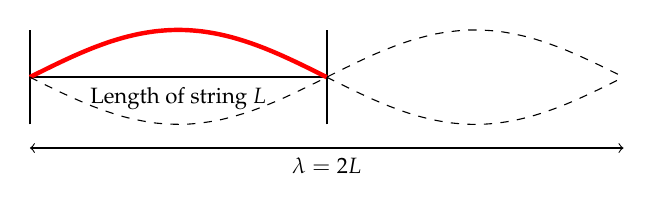
\begin{tikzpicture}[scale=1.2]
        \draw[thick](0,0) -- (pi,0)
        node[midway,below]{\footnotesize Length of string $L$};
        \draw[thick](0,-.5) --(0,.5);
        \draw[thick](pi,-.5)--(pi,.5);
        \draw[smooth,samples=20,domain=0:pi,red,ultra thick]
        plot({\x},{0.5*sin(180/pi*\x)});
        \draw[smooth,samples=20,domain=pi:2*pi,dashed]
        plot({\x},{0.5*sin(180/pi*\x)});
        \draw[smooth,samples=20,domain=0:2*pi,dashed]
        plot({\x},{-.5*sin(180/pi*\x)});
        \draw[<->](0,-.75)--(2*pi,-.75)
        node[midway,below]{\footnotesize $\lambda=2L$};
      \end{tikzpicture}
    \end{center}
  \end{itemize}
\end{frame}


\begin{frame}{Fundamental Frequency of a Wave on a String}
  Using the universal wave equation we can relate the fundamental frequency
  $f_1$ to the speed of a traveling wave along the string $v_\mathrm{str}$:

  \eq{-.2in}{
    \boxed{f_1=\frac{v_\mathrm{str}}{\lambda}=\frac{v_\mathrm{str}}{2L}}
  }
\end{frame}


\begin{frame}
  \frametitle{Standing Waves On a String Length $L$}
  
  A second resonance frequency occurs when $L=\lambda$:
  \vspace{.1in}\begin{columns}
    \column{.45\textwidth}
    \centering
    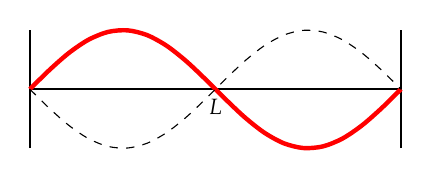
\begin{tikzpicture}[scale=1.5]
      \draw[thick](0,0)--(pi,0)  node[pos=0.5,below]{\footnotesize $L$};
      \draw[thick](0,-.5) --(0,.5);
      \draw[thick](pi,-.5)--(pi,.5);
      \draw[smooth,samples=20,domain=0:pi,red,ultra thick]
      plot({\x},{.5*sin(360/pi*\x)});
      \draw[smooth,samples=20,domain=0:pi,dashed]
      plot({\x},{-.5*sin(360/pi*\x)});
    \end{tikzpicture}
    
    \column{.55\textwidth}
    \eq{0in}{
        f_2=\frac{v_\mathrm{str}}{\lambda}=\frac{v_\mathrm{str}}{L}=2f_1
    }
  \end{columns}

  \vspace{.3in}A third resonance frequency occurs at
  $\displaystyle L=\frac{3}{2}\lambda$:

  \vspace{-.1in}\begin{columns}
    \column{.45\textwidth}
    \centering
    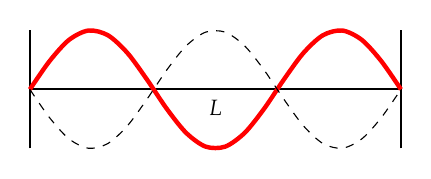
\begin{tikzpicture}[scale=1.5]
      \draw[thick](0,0) -- (pi,0)  node[pos=0.5,below]{\footnotesize $L$};
      \draw[thick](0,-.5) --(0,.5);
      \draw[thick](pi,-.5)--(pi,.5);
      \draw[smooth,samples=20,domain=0:pi,red,ultra thick]
      plot({\x},{.5*sin(540/pi*\x)});
      \draw[smooth,samples=20,domain=0:pi,dashed]
      plot({\x},{-.5*sin(540/pi*\x)});
    \end{tikzpicture}
    
    \column{.55\textwidth}
      
    \eq{0in}{
      f_3=\frac{3v_\mathrm{str}}{2L}=3f_1
    }
  \end{columns}
\end{frame}



\begin{frame}
  \frametitle{Standing Waves On a String Length $L$}
  The $n$-th resonance frequency of a wave on string is just whole-number
  multiples of the fundamental frequency:
  
  \eq{-.3in}{
    \boxed{f_n=nf_1}\quad n=1,2,3,\ldots %\quad
    %\text{\normalsize (standing wave on string)}
  }

  \vspace{-.15in}This equation is \emph{identical} to the harmonic frequencies,
  meaning that every harmonic is a resonance frequency. Standing waves on a
  string have a \emph{full set of harmonics}.
  
  \vspace{.25in}The wavelengths corresponding to the resonance frequencies are:

  \eq{-.2in}{
      \boxed{\lambda=\frac{2L}{n}}\quad n=1,2,3,\ldots
    }
\end{frame}


%\begin{frame}
%  \frametitle{Transfer of Sound Wave}
%  Example: tuning fork
%  
%  \pic{.9}{tuningfork.jpg}
%\end{frame}
%
%\begin{frame}
%  \frametitle{Transfer of Sound Wave}
%  \framesubtitle{Schematic Diagram vs.\ Wave Graph}
%  We can also express the amplitude of the sound wave by plotting the change in
%  \emph{air pressure}:
%
%  \vspace{-.2in}
%  \begin{center}
%    \pic{.9}{schematic-vs-graph.png}
%  \end{center}
%\end{frame}



\section{Sound Waves}

\begin{frame}{Transfer of Sound Wave in Air}
  Sound wave is a \emph{longitudinal wave}, caused by the compression and
  rarefaction (expansion) of the air molecules. Example: speakers
  \begin{center}
    \vspace{-.1in}\pic{.5}{speaker.jpg}
  \end{center}
  Example: tuning fork
    \begin{center}
    \vspace{-.1in}\pic{.5}{tuningfork.jpg}
  \end{center}
\end{frame}

\begin{frame}{Propagation of Sound Wave}
  \framesubtitle{Schematic Diagram vs.\ Wave Graph}
  We can also express the amplitude of the sound wave by plotting the change in
  \emph{air pressure}:
  \begin{center}
    \vspace{-.2in}\pic{.6}{schematic-vs-graph.png}
  \end{center}
  The sinusoidal shape of the pressure (or density) distribution is how sound
  waves are visualized.
\end{frame}


\begin{frame}{Speed of Sound in a Gas}
  The equation for the speed of sound in a gas (e.g.\ air) is given by:

  \eq{-.2in}{
    \boxed{v_s=\sqrt{\frac{\gamma RT}{M}}}
  }
  \begin{center}
    \begin{tabular}{l|c|l}
      \rowcolor{pink}
      \textbf{Quantity} & \textbf{Symbol} & \textbf{SI Unit} \\ \hline
      Speed of sound         & $v_s$ & \si{m/s}\\
      Temperature            & $T$  & \si{\kelvin}\\
      Universal gas constant & $R$  & \si{J/mol.K}\\
      Molar mass             & $M$  & \si{\kilo\gram/mol}\\
      Adiabatic constant     & $\gamma$  & (no units)
    \end{tabular}
  \end{center}
  For diatomic gases such as air $\gamma=1.4$, and
  $M=\SI{29e-3}{\kilo\gram/mol}$.
\end{frame}



\begin{frame}{Speed of Sound in Air}
  We can \emph{linearize} the speed of sound equation near room temperature
  (about \SI{300}{\kelvin}) using a method called
  \emph{least-square approximation}, which gives us a handy equation for the
  speed of sound:
  
  \eq{-.3in}{ v_s=331 + 0.59T_C
  }
  \begin{center}
    \begin{tabular}{l|c|l}
      \rowcolor{pink}
      \textbf{Quantity} & \textbf{Symbol} & \textbf{SI Unit} \\ \hline
      Speed of sound     & $v_s$ & \si{m/s}\\
      Temperature of air in Celsius & $T_c$ & 
    \end{tabular}
  \end{center}
  Note that this approximate equation only works with air at/near room
  temperature.
\end{frame}


\begin{frame}{Speed of Sound in Different Media}
  \begin{columns}
    \column{.6\textwidth}
    Speed of sound in a liquid depends on the ``bulk modulus'' $K$ and density
    $\rho$ of the liquid:
      
    \eq{-.2in}{ v = \sqrt{\frac{K}{\rho}} }
   
    Speed of sound in a solid depends on the ``Young's modulus'' $E$ of the
    solid and density $\rho$

    \eq{-.2in}{
      v = \sqrt{\frac{E}{\rho}}
    }
    %In general, sound travels fastest in solids, then liquids, then gasses.
    
    \column{.4\textwidth}
    \begin{tabular}{l|c}
      \rowcolor{blue!30}
      \textbf{Material} & \textbf{Speed} (\si{m/s}) \\
      \rowcolor{pink!70}
      \multicolumn{2}{c}{Gases (\SI{0}{\celsius}, \SI{101}{\kilo\pascal})} \\
      Carbon dioxide & 259 \\
      Oxygen         & 316 \\
      Air            & 331 \\
      Helium         & 965 \\
      \rowcolor{pink!70}
      \multicolumn{2}{c}{Liquids (\SI{20}{\celsius})} \\
      Ethanol        & 1162 \\
      Fresh water    & 1482 \\
      Seawater       & 1440-1500 \\
      \rowcolor{pink!70}
      \multicolumn{2}{c}{Solids} \\
      Copper         & 5010 \\
      Glass          & 5640 \\
      Steel          & 5960
    \end{tabular}
  \end{columns}
\end{frame}


%%\begin{frame}
%%  \frametitle{Example Problem}
%%  \textbf{Example 1}: Suppose the room temperature of a classroom is
%%  \SI{21}{\celsius}. Calculate the speed of sound in the classroom. (Use the
%%  simpler equation.)
%%\end{frame}
%%
%%
%%\begin{frame}
%%  \frametitle{Example Problem}
%%  \textbf{Example 2}: The temperature was \SI{4.0}{\celsius} one morning as
%%  Martita hiked through a canyon. She shouted at the canyon wall, and
%%  \SI{2.8}{\second} later heard an echo. How far away was the canyon wall?
%%\end{frame}



\begin{frame}{Mach Number}
  When dealing with sound waves, it is often useful to express speed in terms
  of its ratio to the speed of sound. This ratio is called the
  \textbf{Mach number}\footnote{named after German engineer Ernst Mach}:
  
  \eq{-.2in}{
    \boxed{M=\frac{v}{v_s}}
  }
  \begin{center}
    \begin{tabular}{l|c|l}
      \rowcolor{pink}
      \textbf{Quantity} & \textbf{Symbol} & \textbf{SI Unit} \\ \hline
      Mach Number         & $M$   & no units \\
      Speed of the object & $v$   & \si{m/s} \\
      Local speed of sound & $v_s$ & \si{m/s}
    \end{tabular}
  \end{center}
  \begin{itemize}
  \item When an object is traveling at $M<1$, it is traveling at a
    \emph{subsonic} speed
  \item When an object is traveling at $M>1$, it is traveling at a
    \emph{supersonic} speed
  \end{itemize}
\end{frame}



\begin{frame}{Sound from a Moving Source}
  When a sound is emitted from a point source, the sound wave moves radially
  outward from the point of origin. In this diagram, the source is stationary:
  \begin{center}
    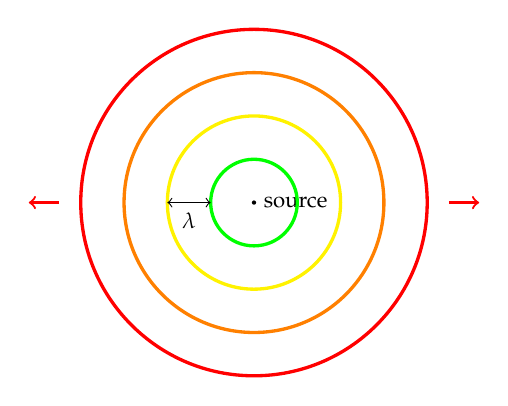
\begin{tikzpicture}[scale=.55]
      \fill[black](0,0) circle(.05) node[right]{\footnotesize source};
      \begin{scope}[very thick]
        \draw[green] (0,0) circle(1);
        \draw[yellow](0,0) circle(2);
        \draw[orange](0,0) circle(3);
        \draw[red]   (0,0) circle(4);
      \end{scope}
      \draw[<->](-1,0)--(-2,0) node[midway,below]{\footnotesize $\lambda$};
      \draw[thick,->,red](4.5,0)--(5.2,0);
      \draw[thick,->,red](-4.5,0)--(-5.2,0);
    \end{tikzpicture}
  \end{center}
  As the wave front moves away from the point source, its area increases (think
  3D), therefore the sound is not as loud.
\end{frame}


\section[Doppler]{Doppler Effect}

\begin{frame}{Sound from a Moving Source}
  But when sound is emitted from a \emph{moving} source, the diagram looks
  different. In this case, the sound source is moving to the right, from $1$ to
  $4$:

  \begin{columns}    
    \column{.4\textwidth}
    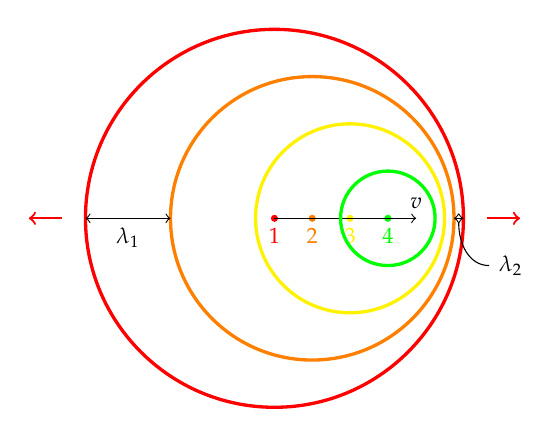
\begin{tikzpicture}[scale=.6]
      \fill[red]   ( 0,0)  circle(.075) node[below]{\footnotesize $1$};
      \fill[orange](.8,0)  circle(.075) node[below]{\footnotesize $2$};
      \fill[yellow](1.6,0) circle(.075) node[below]{\footnotesize $3$};
      \fill[green] (2.4,0) circle(.075) node[below]{\footnotesize $4$};
      \draw[->](0,0)--(3,0) node[pos=1,above]{\footnotesize $v$};
      \begin{scope}[very thick]
        \draw[red]   (  0,0) circle(4);
        \draw[orange]( .8,0) circle(3);
        \draw[yellow](1.6,0) circle(2);
        \draw[green] (2.4,0) circle(1);
      \end{scope}
      \draw[<->](-4,0)--(-2.2,0) node[midway,below]{\footnotesize $\lambda_1$};
      \draw[<->](4,0)--(3.8,0);
      \node (a) at (5,-1) {\footnotesize $\lambda_2$};
      \draw(3.9,-.1) to[out=270,in=180] (a);
      \draw[thick,->,red](4.5,0)--(5.2,0);
      \draw[thick,->,red](-4.5,0)--(-5.2,0);
    \end{tikzpicture}
      
    \column{.6\textwidth}
    \begin{itemize}
    \item When the source is moving \emph{toward you}, the wavelength
      $\lambda_2$ decreases, and the frequency increases.
    \item When the source is moving \emph{away from you}, the wavelength
      $\lambda_1$ increases, and the frequency decreases.
    \end{itemize}
    \vspace{.15in}This is called the \textbf{Doppler effect}. The most
    common example is of an ambulance/police siren as the vehicle approaches
    you.
  \end{columns}
\end{frame}


\begin{frame}{Doppler Effect}
  When a wave source is moving at a speed $v_{\textrm{src}}$ and the observer is
  moving at $v_{\textrm{ob}}$, the frequency perceived by the observer is
  shifted to $f'$:

  \eq{-.2in}{
    \boxed{f'=\frac{v_s+v_{\textrm{ob}}}{v_s-v_{\textrm{src}}}f}
  }
  \begin{center}
    \begin{tabular}{l|c|l}
      \rowcolor{pink}
      \textbf{Quantity} & \textbf{Symbol} & \textbf{SI Unit} \\ \hline
      Apparent frequency  & $f'$   & \si{hertz} (hertz) \\
      Actual frequency    & $f$    & \si{hertz} (hertz) \\
      Speed of sound      & $v_s$ & \si{m/s} (meters per second) \\
      Speed of source & $v_{\textrm{src}}$ & \si{m/s} (meters per second)\\
      Speed of observer & $v_{\textrm{ob}}$ & \si{m/s} (meters per second)
    \end{tabular}
  \end{center}
\end{frame}


\begin{frame}{Sound from a Source Moving At Sonic Speed}
  Doppler effect is more interesting is when the sound source is moving at the
  speed of sound ($M=1$):
  \vspace{.2in}
  \begin{columns}
    
    \column{.4\textwidth}
    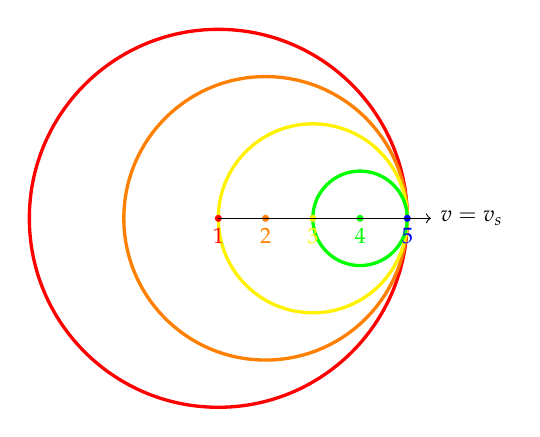
\begin{tikzpicture}[scale=.6]
      \begin{scope}[very thick]
        \draw[red]   (0,0) circle(4);
        \draw[orange](1,0) circle(3);
        \draw[yellow](2,0) circle(2);
        \draw[green] (3,0) circle(1);
      \end{scope}
      \fill[red]   (0,0) circle(.075) node[below]{\footnotesize $1$};
      \fill[orange](1,0) circle(.075) node[below]{\footnotesize $2$};
      \fill[yellow](2,0) circle(.075) node[below]{\footnotesize $3$};
      \fill[green] (3,0) circle(.075) node[below]{\footnotesize $4$};
      \fill[blue]  (4,0) circle(.075) node[below]{\footnotesize $5$};
      \draw[->](0,0)--(4.5,0) node[pos=1,right]{\footnotesize $v=v_s$};
    \end{tikzpicture}
      
    \column{.6\textwidth}
    \begin{itemize}
    \item The wave fronts (crests) from all the waves are bunched up just in
      front of the source
    \item Since sound wave is a pressure wave, right in front of the sound
      source, there is a large change in pressure (called a shock wave)
    \item When the shock passes an observer, an loud bang can be heard (aka
      \textbf{sonic boom})
    \end{itemize}
  \end{columns}
\end{frame}



\begin{frame}{Sound from a Supersonic Source}
  When the sound source is moving at $M>1$:
  \begin{columns}
    \column{.47\textwidth}
    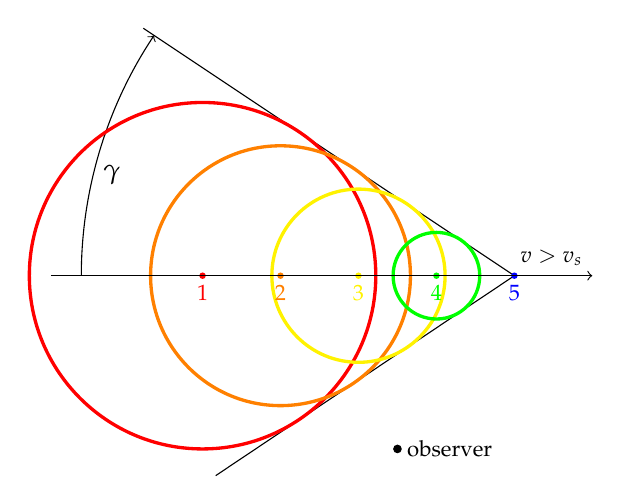
\begin{tikzpicture}[scale=.55]
      \draw[rotate around={213.8:(7.2,0)}](7.2,0)--(15.5,0);
      \draw[rotate around={146.3:(7.2,0)}](7.2,0)--(17.5,0);
      \draw[->](-2.8,0) arc(180:146.3:10) node[pos=.4,right]{$\gamma$};
      \begin{scope}[very thick]
        \draw[red]   (0,0) circle(4);
        \draw[orange](1.8,0) circle(3);
        \draw[yellow](3.6,0) circle(2);
        \draw[green] (5.4,0) circle(1);
      \end{scope}
      \fill[red]   (0,0) circle(.075) node[below]{\footnotesize $1$};
      \fill[orange](1.8,0) circle(.075) node[below]{\footnotesize $2$};
      \fill[yellow](3.6,0) circle(.075) node[below]{\footnotesize $3$};
      \fill[green] (5.4,0) circle(.075) node[below]{\footnotesize $4$};
      \fill[blue]  (7.2,0) circle(.075) node[below]{\footnotesize $5$};
      \draw[->](-3.5,0)--(9,0) node[pos=1,above left]{\footnotesize $v>v_s$};
      \fill[black](4.5,-4) circle(.1) node[right]{\footnotesize observer};
    \end{tikzpicture}
      
    \column{.53\textwidth}
    An \emph{oblique shock} is formed at an angle (called the
    \textbf{Mach angle}) given by:
      
    \eq{-.2in}{
      \gamma=\sin^{-1}\left(\frac{1}{M}\right)
    }

    \vspace{-.15in}A stationary observer does not hear the sound source coming
    until it has gone past!
  \end{columns}
\end{frame}


\begin{frame}{Bullet in Supersonic Flight}
  Generating a shock wave does not require an actual sound source. \emph{Any}
  object moving through air creates a pressure disturbance. For example, this
  is a bullet in supersonic flight:
  \begin{center}
    \pic{.3}{bullet2.jpg}
  \end{center}
\end{frame}


\begin{frame}{Duck in Water}
  Shock waves are not confined to sound waves only. In this example, a duck
  swims faster than the speed of the water wave, and it also creates a cone
  shape.
  \begin{center}
    \pic{.5}{duck.jpg}
  \end{center}
\end{frame}


\section{Sound}

\begin{frame}{Beat Frequency}
%  The principle of superposition of waves means that when two or more waves are
%  present, the \emph{total} wave is just the \emph{sum} of the waves. The
%  consequence of superposition is
%  \begin{itemize}
%  \item Constructive interference
%  \item Destructive interference
%  \end{itemize}
  When waves (e.g.\ sound waves) of two different frequencies are added
  together, there is both constructive and destructive interference because of
  the principle of superposition
  \begin{itemize}
  \item Plotting two functions representing two waves with equal magnitude
    and wave speed $v_s$: $\color{blue}{y=\sin(x)}$
    \uncover<2->{and $\color{red}{y=\sin(1.1x)}$}
  \end{itemize}
  \begin{center}
    \vspace{-.1in}
    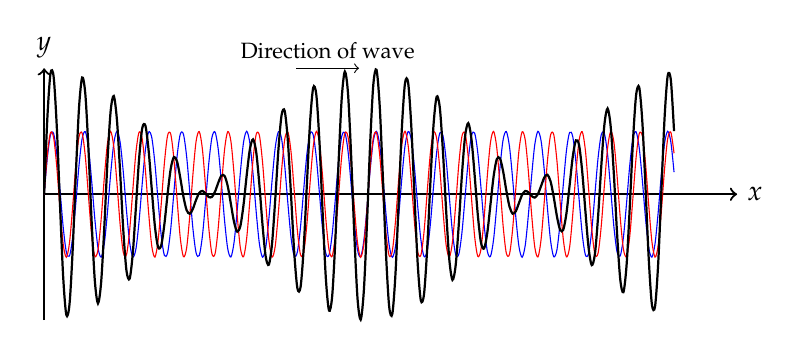
\begin{tikzpicture}[scale=.8]
      \draw[->,thick](0,0) --(11,0) node[pos=1,right] {$x$};
      \draw[->,thick](0,-2)-- (0,2) node[pos=1,above] {$y$};
      \draw[->](4,2)--(5,2) node[midway,above]{\footnotesize Direction of wave};
      \uncover<1,3->{
        \draw[blue,smooth,samples=200,domain=0:10] plot({\x},{sin(700*\x)});
      }
      \uncover<2->{
        \draw[smooth,samples=200,domain=0:10,red] plot({\x},{sin(770*\x)});
      }
      \uncover<4>{
        \draw[smooth,samples=200,domain=0:10,thick]
        plot({\x},{sin(700*\x)+sin(770*\x)});
      }
    \end{tikzpicture}
  \end{center}
  \uncover<4->{
    \vspace{-.1in}
    \begin{itemize}
    \item The thick black line is the sum: $y=\sin(x) + \sin(1.1x)$
    \end{itemize}
  }
\end{frame}



\begin{frame}
  \frametitle{Beat Frequency}
  The \textbf{beat frequency} is the absolute difference of the frequencies of
  the two component waves:

  \eq{-.2in}{
    \boxed{f_\mathrm{beat}=|f_1-f_2|}
  }
  \begin{center}
    \begin{tabular}{l|c|l}
      \rowcolor{pink}
      \textbf{Quantity} & \textbf{Symbol} & \textbf{SI Unit} \\ \hline
      Beat frequency     & $f_\mathrm{beat}$   & \si{\hertz} (hertz) \\
      Frequency of 1st component wave & $f_1$ & \si{\hertz} (hertz) \\
      Frequency of 2nd component wave & $f_2$ & \si{\hertz} (hertz)
    \end{tabular}
  \end{center}
  For sound waves, they sound like a pulsating ``whoomf''. Musicians often use
  the beat frequencies to determine whether someone is play in tune or out of
  tune.
\end{frame}



\section[Pipes]{Standing Waves in Pipes}

\begin{frame}{Standing Waves in a Closed Pipe}
  We have already studied standing-wave patterns on a``vibrating string''.
  Standing-wave patterns of sound waves can be found on pipes that have both
  ends closed:
  \begin{center}
    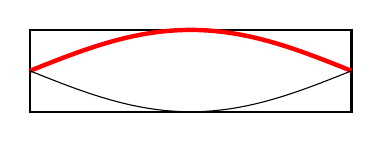
\begin{tikzpicture}[scale=1.3,yscale=.4]
      \draw[thick](0,-1) rectangle(pi,1);
      \draw[smooth,samples=20,domain=0:pi,red,ultra thick]
      plot({\x},{sin(180/pi*\x)});
      \draw[smooth,samples=20,domain=0:pi] plot({\x},{-1*sin(180/pi*\x)});
    \end{tikzpicture}
    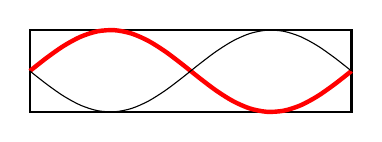
\begin{tikzpicture}[scale=1.3,yscale=.4]
      \draw[thick](0,-1) rectangle(pi,1);
      \draw[smooth,samples=20,domain=0:pi,red,ultra thick]
      plot({\x},{sin(360/pi*\x)});
      \draw[smooth,samples=20,domain=0:pi] plot({\x},{-1*sin(360/pi*\x)});
    \end{tikzpicture}\\
    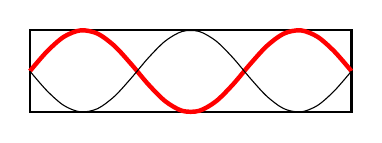
\begin{tikzpicture}[scale=1.3,yscale=.4]
      \draw[thick](0,-1) rectangle(pi,1);
      \draw[smooth,samples=20,domain=0:pi,red,ultra thick]
      plot({\x},{sin(540/pi*\x)});
      \draw[smooth,samples=20,domain=0:pi] plot({\x},{-1*sin(540/pi*\x)});
    \end{tikzpicture}
    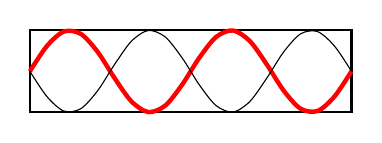
\begin{tikzpicture}[scale=1.3,yscale=.4]
      \draw[thick](0,-1) rectangle(pi,1);
      \draw[smooth,samples=20,domain=0:pi,red,ultra thick]
      plot({\x},{sin(720/pi*\x)});
      \draw[smooth,samples=20,domain=0:pi] plot({\x},{-1*sin(720/pi*\x)});
    \end{tikzpicture}
  \end{center}
  The air molecules at the end of the pipe cannot vibrate along the direction of
  wave motion, therefore they have to be nodes. This pattern is identical to
  that of the vibrating string.
\end{frame}


\begin{frame}{Standing Waves in Closed Pipes}
  Like strings, pipes that are \emph{closed at both ends} have resonance
  frequencies that are whole-number multiple of the fundamental frequency $f_1$:
  
  \eq{-.2in}{
    \boxed{f_n=nf_1=n\frac{v_s}{2L}}\quad n=1,2,3,\ldots
  }
  
  And the wavelengths corresponding to the resonance frequencies are:

  \eq{-.2in}{
    \boxed{\lambda=\frac{2L}{n}}\quad n=1,2,3,\ldots
  }

  The difference between a closed pipe and a string is that the wave speed is
  now the speed of sound $v_s$ inside the pipe.
\end{frame}



\begin{frame}{Standing Waves in Open Pipes}
  Many types of organ pipes, as well as the flute, can be modelled as pipes
  that are open on both ends. The standing-wave patterns for open pipes are
  similar to strings and closed pipes, but with nodes and anti-nodes reversed:
  \begin{center}
    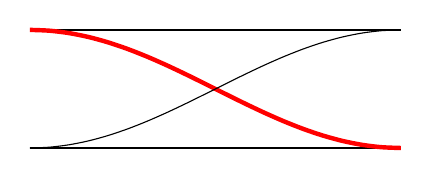
\begin{tikzpicture}[scale=1.5]
      \draw[thick](0,-.5)--(pi,-.5);
      \draw[thick](0,0.5)--(pi,0.5);
      \draw[smooth,samples=20,domain=0:pi,red,ultra thick]
         plot({\x},{0.5*sin(180/pi*\x+90)});
      \draw[smooth,samples=20,domain=0:pi]
        plot({\x},{-.5*sin(180/pi*\x+90)});
    \end{tikzpicture}
    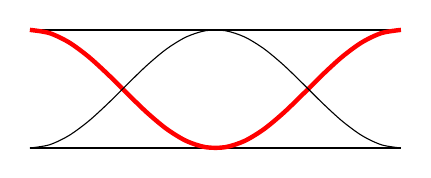
\begin{tikzpicture}[scale=1.5]
      \draw[thick](0,-.5)--(pi,-.5);
      \draw[thick](0,0.5)--(pi,0.5);
      \draw[smooth,samples=20,domain=0:pi,red,ultra thick]
        plot({\x},{0.5*sin(360/pi*\x+90)});
      \draw[smooth,samples=20,domain=0:pi]
        plot({\x},{-.5*sin(360/pi*\x+90)});
    \end{tikzpicture}\\
    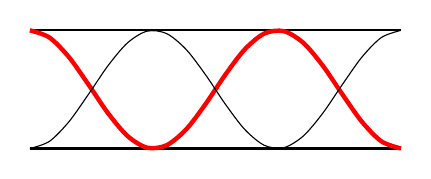
\begin{tikzpicture}[scale=1.5]
      \draw[thick](0,-.5)--(pi,-.5);
      \draw[thick](0,0.5)--(pi,0.5);
      \draw[smooth,samples=20,domain=0:pi,red,ultra thick]
      plot({\x},{0.5*sin(540/pi*\x+90)});
      \draw[smooth,samples=20,domain=0:pi]
      plot({\x},{-.5*sin(540/pi*\x+90)});
    \end{tikzpicture}
    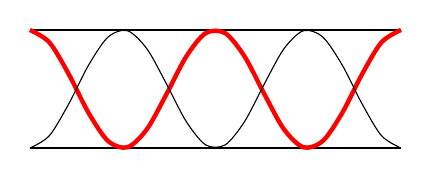
\begin{tikzpicture}[scale=1.5]
      \draw[thick](0,-.5)--(pi,-.5);
      \draw[thick](0,0.5)--(pi,0.5);
      \draw[smooth,samples=20,domain=0:pi,red,ultra thick]
      plot({\x},{0.5*sin(720/pi*\x+90)});
      \draw[smooth,samples=20,domain=0:pi]
      plot({\x},{-.5*sin(720/pi*\x+90)});
    \end{tikzpicture}
  \end{center}
  The air molecules at the ends of the pipe have maximum vibrations, and are
  anti-nodes in the standing wave.
%  \begin{columns}
%    \column{.5\textwidth}
%    First resonance at $\lambda=2L$
%    \begin{displaymath}
%      f_1=\frac{v_s}{\lambda}=\frac{v_s}{2L}
%    \end{displaymath}
%    \column{.5\textwidth}
%    Second resonance at $\lambda=L$
%    \begin{displaymath}
%      f_2=\frac{v_s}{\lambda}=\frac{v_s}{L}=2f_1
%    \end{displaymath}
%  \end{columns}
\end{frame}



\begin{frame}{Standing Waves in Open Pipes}
  Not surprisingly, like strings and closed pipes, open pipes have resonance
  frequencies that are whole-number multiple of the fundamental frequency $f_1$:
  
  \eq{-.2in}{
    \boxed{f_n=nf_1=n\frac{v_s}{2L}}\quad n=1,2,3,\ldots
  }
  
  And the wavelengths corresponding to the resonance frequencies are also
  identical to that of the closed pipes.

  \eq{-.2in}{
    \boxed{\lambda=\frac{2L}{n}}\quad n=1,2,3,\ldots
  }
  Strings, closed pipes and open pipes are all said to have
  ``full set of harmonics'' because every harmonic frequency is also a
  resonance frequency.
\end{frame}


\begin{frame}{Standing Waves in Semi-Open Pipes}
  %\framesubtitle{This is when things get a bit more interesting\ldots}
  However, most organ pipes, woodwind and brass instruments are in fact
  modelled as pipes that are \emph{closed at one end and open at the other}
%  \begin{itemize}
%  \item Examples: Most organ pipes, clarinet, oboes, brass instruments
%  \end{itemize}
  \begin{center}
    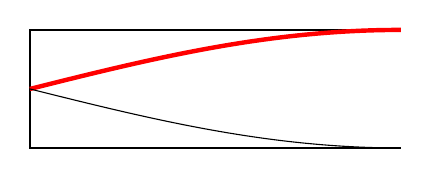
\begin{tikzpicture}[scale=1.5]
      \draw[thick](pi,-.5)--(0,-.5)--(0,.5)--(pi,.5);
      \draw[smooth,samples=20,domain=0:pi,red,ultra thick]
         plot({\x},{0.5*sin(90/pi*\x)});
      \draw[smooth,samples=20,domain=0:pi]
        plot({\x},{-.5*sin(90/pi*\x)});
    \end{tikzpicture}
    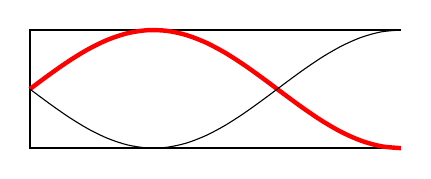
\begin{tikzpicture}[scale=1.5]
      \draw[thick](pi,-.5)--(0,-.5)--(0,.5)--(pi,.5);
      \draw[smooth,samples=20,domain=0:pi,red,ultra thick]
        plot({\x},{0.5*sin(270/pi*\x)});
      \draw[smooth,samples=20,domain=0:pi]
        plot({\x},{-.5*sin(270/pi*\x)});
    \end{tikzpicture}\\
    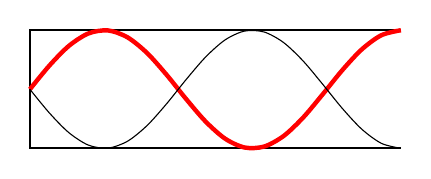
\begin{tikzpicture}[scale=1.5]
      \draw[thick](pi,-.5)--(0,-.5)--(0,.5)--(pi,.5);
      \draw[smooth,samples=20,domain=0:pi,red,ultra thick]
      plot({\x},{0.5*sin(450/pi*\x)});
      \draw[smooth,samples=20,domain=0:pi]
      plot({\x},{-.5*sin(450/pi*\x)});
    \end{tikzpicture}
    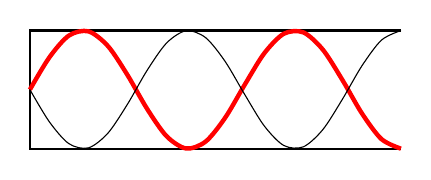
\begin{tikzpicture}[scale=1.5]
      \draw[thick](pi,-.5)--(0,-.5)--(0,.5)--(pi,.5);
      \draw[smooth,samples=20,domain=0:pi,red,ultra thick]
      plot({\x},{0.5*sin(630/pi*\x)});
      \draw[smooth,samples=20,domain=0:pi]
      plot({\x},{-.5*sin(630/pi*\x)});
    \end{tikzpicture}
  \end{center}
  The closed end is a node (like in the closed pipes), while the open end is
  an anti-node (like in the open pipes).

\end{frame}

\begin{frame}
  \frametitle{Standing Waves in Semi-Open Pipes}
  Again starting with the fundamental frequency (lowest frequency where a
  standing wave can form inside the pipe). This occurs at $\lambda=4L$:

  \vspace{-.1in}
  \begin{center}
    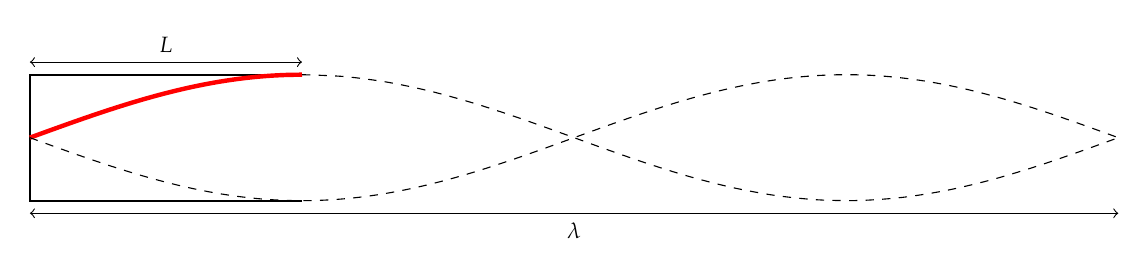
\begin{tikzpicture}[xscale=1.1,yscale=.8]
      \draw[thick](pi,-1)--(0,-1)--(0,1)--(pi,1);
      \draw[smooth,samples=20,domain=0:pi,red,ultra thick]
      plot({\x},{sin(90/pi*\x)});
      \draw[smooth,samples=20,domain=pi:4*pi,dashed]
      plot({\x},{sin(90/pi*\x)});
      \draw[smooth,samples=80,domain=0:4*pi,dashed]
      plot({\x},{-1*sin(90/pi*\x)});
      \draw[<->](0,1.2)--(pi,1.2)
      node[midway,above]{\footnotesize $L$};
      \draw[<->](0,-1.2)--(4*pi,-1.2)
      node[midway,below]{\footnotesize $\lambda$};
    \end{tikzpicture}
  \end{center}
  
  Fundamental frequency $f_1$ differs from the open-pipe and closed-pipe
  configurations by a factor of 2:

  \eq{-.2in}{
    \boxed{f_1=\frac{v_s}{\lambda}=\frac{v_s}{4L}}
  }

\end{frame}

\begin{frame}
  \frametitle{Standing Waves in Semi-Open Pipes}
  Likewise, second resonance can be found at
  $\displaystyle \lambda=\frac{4}{3}L$:
  \begin{columns}
    \column{.45\textwidth}
    \centering
    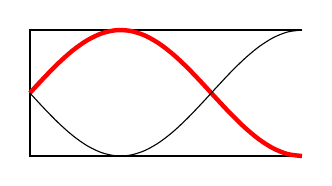
\begin{tikzpicture}[xscale=1.1,yscale=.8]
      \draw[thick](pi,-1)--(0,-1)--(0,1)--(pi,1);
      \draw[smooth,samples=20,domain=0:pi,red,ultra thick]
      plot({\x},{sin(270/pi*\x)});
      \draw[smooth,samples=20,domain=0:pi] plot({\x},{-1*sin(270/pi*\x)});
    \end{tikzpicture}
    
    \column{.55\textwidth}

    \eq{-.4in}{
      f_{\mathrm{res},2}=\frac{v_s}{\lambda}=\frac{3v_s}{4L}=3f_1
    }
  \end{columns}
  And then, third resonance at $\displaystyle \lambda=\frac{4}{5}L$:
  \begin{columns}

    \column{.45\textwidth}
    \centering
    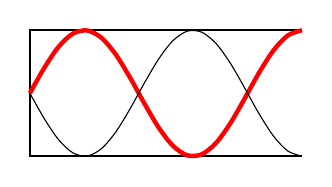
\begin{tikzpicture}[xscale=1.1,yscale=.8]
      \draw[thick](pi,-1)--(0,-1)--(0,1)--(pi,1);
      \draw[smooth,samples=20,domain=0:pi,red,ultra thick]
      plot({\x},{sin(450/pi*\x)});
      \draw[smooth,samples=20,domain=0:pi] plot({\x},{-1*sin(450/pi*\x)});
    \end{tikzpicture}

    \column{.55\textwidth}
    \eq{-.2in}{
      f_{\mathrm{res},3}=\frac{v_s}{\lambda}=\frac{5v_s}{4L}=5f_1
    }
  \end{columns}
\end{frame}

\begin{frame}
  \frametitle{Standing Waves in Semi-Open Pipes}
  Only \textbf{odd-number multiples} of the fundamental frequency are resonance
  frequencies in a semi-open pipe.  We say that semi-open pipes have an
  \emph{odd} set of harmonics.

  \eq{-.25in}{
    \boxed{f_n = (2n-1)f_1=\frac{(2n-1)v_s}{4L}}\quad n=1,2,3,\ldots
  }
  
  Because fundamental frequency $f_1$ is lower than the open-pipe configuration
  by a factor of 2 for the same length $L$, it has advantages when designing an
  organ pipe.
\end{frame}


%\begin{frame}
%  \frametitle{Resonance \emph{Length} in a Semi-Open Pipe}
%  \begin{itemize}
%  \item Now that we have looked at resonance \emph{frequencies}, we'll look
%    at resonance \emph{lengths}
%  \item We produce a single frequency in the pipe, and vary the length of the
%    pipe until we have resonance
%  \end{itemize}
%\end{frame}
%
%\begin{frame}
%  \frametitle{Resonance Length in a Semi-Open Pipe}
%  Let's submerge a part of this pipe in water\ldots
%  \begin{center}
%    \pic{.7}{res-length-closed.png}
%  \end{center}
%\end{frame}
%
%\begin{frame}
%  \frametitle{Resonance Length in a Semi-Open Pipe}
%  The resonance lengths are \textbf{odd whole-number multiples} of the first
%  resonance length $L_1$: %($\displaystyle\frac{\lambda}{4}$):
%  
%  \eq{-.2in}{
%    \boxed{L_{\mathrm{res},n} = (2n-1)L_1}
%    \quad\text{\normalsize where}\quad
%    \boxed{L_1 = \frac{\lambda}{4}}
%  }
%\end{frame}
%
%
%
%\begin{frame}
%  \frametitle{Resonance in an Open Pipe}
%  We can also repeat this with pipes that are open on both ends.
%  \begin{center}
%    \pic{.75}{res-length-open.png}
%  \end{center}
%\end{frame}
%
%
%
%\begin{frame}
%  \frametitle{Resonance in an Open Pipe}
%  Resonance lengths of an open pipe are \textbf{whole-number multiples} of the
%  first resonance length $L_1$:
%
%  \eq{-.25in}{
%    \boxed{L_{\mathrm{res},n}=nL_1}
%    \quad\text{\normalsize (open pipe)}
%  }
%  
%  \vspace{-.1in}where first resonance length is given by:
%  
%  \eq{-.2in}{
%    \boxed{L_1=\frac{\lambda}{2}}
%  }
%  
%  Be careful! This equation looks a lot like the resonance frequency equation!
%\end{frame}
%
\end{document}
